\subsection{Hierarchische Baumstrukturen}\label{subsec:htrees}

\begin{center}
    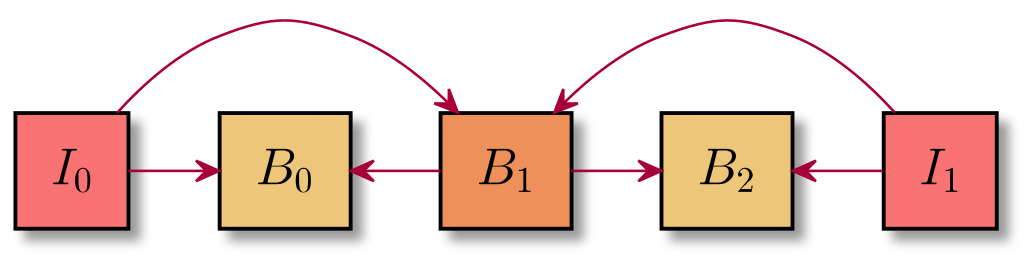
\includegraphics[width=0.75\textwidth]{../img/b-pictures}
\end{center}

\noindent Um mehrere Ansichten zu Kodieren, verwenden wir hierarchische Baumstrukturen~\cite{hier-b-frames} von B-Rahmen.
Wie im Bild zu sehen, werden hier zun\"achst B-Rahmen aus Paaren von I-Rahmen erzeugt und daraus weitere B-Rahmen, usw.


\subsubsection{Hierarchische Baumstruktur f\"ur mehrere Ansichten}
\begin{center}
    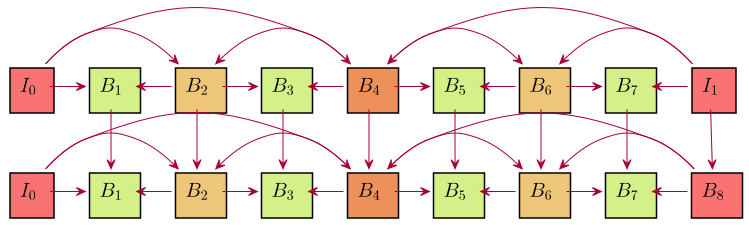
\includegraphics[width=1\textwidth]{../img/b-pictures-3d}
\end{center}
Aus unseren Ergebnissen~(siehe \textit{\nameref{sec:idea}}) k\"onnen wir schlussfolgern, dass unsere Kodierungsstruktur
sowohl r\"aumliche als auch zeitliche Nachbarn zum Produzieren eines B-Rahmens verwenden sollte.
Es ist zu sehen, dass B-Rahmen der Nachbaransicht hier parallel und identisch zur ersten Ansicht erzeugt werden.
Allerdings wird in der Zweiten zus\"atzlich die erste Ansicht zum Erzeugen von B-Rahmen eingebunden.

\noindent\newline \texttt{H.264} erlaubt es uns sogar f\"ur einzelne Macrobl\"ocke die Rahmen zu definieren~\cite{h264},
aus welchen sie erzeugt werden.
Somit bleiben wir flexibel und k\"onnen entscheiden, ob wir r\"aumliche oder zeitliche Nachbarn einbinden.
